\documentclass[a4paper,12pt]{article}
\usepackage[russian]{babel} 
\usepackage[utf8x]{inputenc}
\usepackage{graphicx}


\begin{document}
\begin{titlepage}
\begin{center} 
\large Ульяновский Государственный Университет\\[4.5cm] 

\huge Доклад по философии\\[0.6cm] 
\large на~тему \textbf{<<Неоплатонизм>>}\\[1.7cm]
\begin{center}
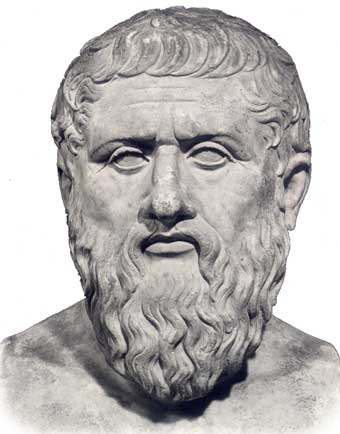
\includegraphics[scale=0.5]{images/platon.jpg}
\end{center}
\end{center} 
\begin{minipage}{0.5\textwidth}
\begin{flushleft}
\vspace{20 mm}
\emph{Автор:} Кузнецов Юрий Игоревич\\
\emph{Группа:} МОТС 41\\
\emph{Факультет:} ФМиИТ\\
\end{flushleft}
\end{minipage}
\thispagestyle{empty}
\end{titlepage} 
\newpage
\tableofcontents
\newpage

\part{Введение}
Последней крупной  философской системой западной античности является неоплатонизм. Философия неоплатонизма возникает в \textbf{III} н. э. и развивается вплоть до начала \textbf{VII} в. Неоплатонизм связан, прежде всего, с именами \textit{Плотина}, \textit{Порфирия}, \textit{Прокла} и \textit{Ямвлиха}. Характерно, что возврат к идеям Платона и потребность в их переосмыслении возникают в период, когда античный способ философствования подходит к концу, постепенно уступая новому и радикально отличному от него, философствованию, отправляющемуся от христианского Откровения. Неоплатонизм возникает на фоне широкого распространения эклектических учений, пытающихся сочетать в себе несоединимые элементы древних философских систем.\\

\medskip
Подобно тому, как стоицизм был характерен для теоретического мировоззрения Ранней Римской империи, так для Поздней Римской империи характерен неоплатонизм. Точнее, неоплатонизм возникает не во времена Поздней Римской империи, а в промежутке между Ранней и Поздней империями, в смутное время, когда Ранняя Римская империя почти что перестала существовать, а Поздняя Римская Империя еще не возникла. Иначе говоря, он возникает в вакууме между империями. Этот вакуум продолжался с 235 г., с года, когда был убит солдатами последний представитель династии Северов и до 284 г., когда власть в восстановившейся десятью годами ранее Римской империи жестко взял в свои руки \textit{Диоклетиан}, введший новую форму высшего правления по типу восточных \textit{деспотий}, \textit{доминат}.
\newpage
\part{Основоположник}
\begin{center}
\textbf{\textit{Плотин (204/205 – 270 гг.)}}
\end{center}
Плотин родился в римской провинции Египта в городе Ликополе. Он учился у ряда философов, которые его не удовлетворяли. Затем он попадает к \textit{Аммонию Саккасу} - известному греческий философу из Александрии. Плотин пробыл учеником Аммония одиннадцать лет, а решил ознакомиться с мировоззрением персов, а если возможно, то и индийцев, и примкнул к войску \textit{Гордиана III}. Военный поход, в котором участвовал Плотин, закончился разгромом римлян. Но основоположнику неоплатонизма все таки удалось спастись. При сменившем Гордиана III \textit{Филиппе Аравитянине} Плотин оказался в Риме, где основал свою школу и возглавлял её в течение четверти века, имея в числе учеников и сенаторов, и самого императора \textit{Галлиена}. Имея на Галлиена большое влияние, Плотин просил о выделении ему территории для реализации социально-политического проекта Платона, для создания Платонополиса. Император практически согласился, но осуществлению этого утопического замысла помешали императорские советники.\\

\medskip
Плотин написал 54 опуса на различные темы.На Плотина оказал значительное влияние Платон. На его мировоззрение также повлияли многие другие греческие и даже римские философы, в том числе Сенека и Аристотель.
\newpage
\part{Монистический идеализм}
Плотин обосновывает своё идеалистическое учение через учение о разных типах людей. Обыденный человек погружен в чувственно-практическое существование. Он весь во внешнем и вещном бытии, потерян и самоунижен в нем. Для такого человека вещи важнее идей, материальное важнее идеального. Для обыденного низменного человека тело важнее души, и он тешит своё тело, нисколько о душе не беспокоясь. Вся деятельность души такого человека обусловлена его пребыванием в теле, целиком зависит от тела.\\

\medskip
Иной, возвышенный человек поднимается от низшего состояния существования к высшему его состоянию. Он переносит центр тяжести своего бытия с телесного на душевное. Он развивает в  себе способности к сверхчувственному интеллектуальному умосозерцанию, он обращается от внешнего мира в глубины своей души и находит там истину, покой и безмятежность, которые столь недоступны низменному человеку. Возвышенный человек отворачивается от чувственной красоты, презирает её и ищет красоту истинную. Прежде всего, он способен увидеть то, что не видит низменный человек: красоту добродетели, благоразумных действий, добрых нравов, красоту величия характера, справедливости сердца и т.п. На этой ступени человеческого бытия душа в своей деятельности все ещё пребывает в теле, но она от тела независима.\\

\medskip
Эту относительную независимость души от тела возвышенного человека Плотин обосновывает идеей о предсуществовании души. Эта душа созерцала и добродетель, и справедливость, и саму красоту в чистом виде как нечто совершенно идеальное, как идею. Оттого она и способна узнать все это в заземлённой и частной, конкретной форме существования.

\newpage
\part{Структура мировой системы}
Мир в представлении Плотина строго иерархичен, он образует ступени нисходящего бытия, начинающегося в сверхбытии. Существование чувственного телесного мира самоочевидно, он дан нашим чувствам, наше тело – часть этого мира, мы его часть. Но относится Плотин к этому миру отрицательно и не считает его единственным, исчерпывающим все возможное бытие. Даже лучшее в этом мире, его несомненная красота, красота, в частности, природы, которая так волнует многих, порождая в их душах великую радость, лишь слабый и тусклый отблеск истинной, сверхтелесной и сверхприродной красоты.\\

\medskip 
Источником красоты является объективный мировой разум. Ведь красота – это гармония и форма. Но в природе форма разделена пространственно на части, и в этой разделённости очень легко утратить единство формы. Красота в природе, красота телесной вещи – в единстве её частей, а это единство – от разума. Следовательно, разум есть нечто иное, чем природа, высшее по отношению к ней начало. 
В природе есть как одушевлённое, так и неодушевлённое. Материальное не может породить душевное. Следовательно, надо допустить иное, чем природа, начало, а именно, мировую душу. Мировая душа не тождественна мировому разуму, потому что душа равно одушевляет и прекрасное, и безобразное, душа равнодушна к красоте. Поскольку прекрасного меньше, чем одушевлённого, то разум дальше от природы и выше, чем мировая душа, ведь его проявление в природе более избирательно.
Один мировой разум не может быть источником красоты, в основе которой лежит единство вещей. Сам по себе разум не содержит в себе единства, он может быть и хаотической совокупностью содержащихся в нем идей. Поэтому Плотин выдвигает в качестве начала ещё и единое. Таким образом, в философии неоплатонизма можно выделить четыре начала: природа, мировая душа, мировой разум и единое.

\newpage
\begin{figure}[h]
	\begin{center}
		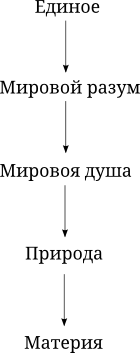
\includegraphics[scale=0.9]{images/sc_ph1.png}
		\caption{Иерархия бытия}
	\end{center}	
\end{figure}
\part{Структура мировой системы}
Все мировоззрение Плотина пронизано единством, до обожествления Единого. Единство, конечно, является важнейшей стороной мироздания и всего, что в нем. Без единства невозможны ни красота, ни жизнь, ни общества. Каждое человеческое общество потому и общество, что в нем есть какое-то единство и взаимное сочувствие.\\

\medskip
Плотин  выносит единое за пределы многого, возвышает его над многим и делает его первичным по отношению ко многому. \textit{Единое} для многого недоступно, многое не способно никак повлиять на единое, заставить его считаться с собой. А само многое к самоорганизации неспособно. Мировая иерархия Плотина есть и отражение социальной иерархии в Римской империи, и предвосхищение феодальной иерархии.
Итак, исторгнутое Плотином из многого единое становится у него Единым. Но, будучи вынесенным за скобки, внутри которых остался весь интеллектуальный, душевный и телесный мир, Единое оказывается в сущности ничем, оно непознаваемо.\\

\medskip
Глубочайшая единственность Единого заключается в том, что оно есть ничто. Плотин, правда, не называет Единое ничем, но в сущности это так. По Плотину, единое, будучи вечным началом всего существующего, само по себе не существует. Во всяком случае, о нем нельзя сказать, что оно существует. Сказать, что Единое существует, – значит его ограничить, поставить рамки, определить. Единое же нельзя заузить, так как оно беспредельно.\\

\medskip 
Плотин взял диалектику единого и многого у Платона и превратил горизонталь «единое – многое» в вертикаль. Единое не познается через многое, потому что единое выше, а многое ниже, а высшее не постигается через низшее, низшее не может быть ключом к пониманию высшего. В высшем всегда есть то, что низшему не доступно, на то оно и высшее.\\

Единое есть абсолютное единство и в том смысле, что не содержит в себе многого, оно, естественно, не содержит в себе и различия, и противоположности, и противоречия.\\

Нет в едином и \textit{субъектно-объектного} отношения, и \textit{саморефлексии}, и самопознания. Единое себя знает, но оно знает себя без познания, потому что познание есть переход от незнания к знанию, что предполагает в качестве исходного состояния состояние незнания, т.е. несовершенства, неполноты, ущербности, недостатка, – а все это чуждо Единому, потому что оно совершенно целостно, самодовлеюще и едино.\\

Единое ни к чему и не стремиться. Ведь всякое стремление также предполагает исходную некую неполноценность, которая должна быть восполнена достижением цели. Единое, ничего не желая и не к чему не стремясь, следовательно, абсолютно счастливо, если под счастьем понимать вечный покой. И в самом деле, в Едином нет времени, оно вневременно. Это нетронутая временем вечность.\\

Плотин сравнивает Единое с Солнцем как источником света и тепла. Он говорит, что Единое есть Благо и Свет и тем самым опять противоречит сам себе.
Говоря о генезисе мира из Единого, Плотин отвергает идею творения мира богом из ничего. Ведь здесь опять-таки бог есть некий деятель, который к чему-то стремиться, чего-то хочет, который как-то даже ограничен своим творением, которое ведь может восстать против своего творца. Плотин понимает творение мира Единым как абсолютно немотивированный объективный процесс. И называть этот процесс принято латинским словом \textit{эманация} (от \textit{emanare} – течь, литься). Но у Плотина текущее, вытекающее Единое не убывает. Оно, творя мир, ничего не утрачивает, оно остается неизбывно целостным, и этот процесс происходит вне времени, от вечности. \\

Единое, будучи светом, светит вокруг себя, оно сияет. Единое не может не производить вокруг себя освещенность, которая, как и всякий свет, убывает по мере удаления от своего источника. Свет светит необходимо. И Единое также производит все иное, чем оно, необходимо. Идея необходимости Плотина состоит в том, что высшее порождает низшее, а низшее должно быть порождено высшим.

\part{Мировой разум}

Первым, что с необходимостью происходит от Единого, есть Ум (Нус). В отличие от небытийного Единого Ум бытиен. Ум у Плотина и аристотелевский бог как само себя мыслящее мышление, и платоновский демиург, который, однако, не имеет перед собой идей, как нечто ему заданное в качестве образцов, а содержит их в себе как свое внутреннее состояние. \\
Ум не только бытиен, но и множествен в том смысле, что в нем существует многое как идеально многое, как множество идей. Ум имеет две стороны: ту, которая обращена к Единому, и ту, которая отвращена от Единого. Как обращенное к Единому Ум един. Как отвращенное от Единого Ум множествен. В целом же Ум есть саморефлексия систематизированной совокупности идей. Ум, в отличие от Единого, делится на познающее и познаваемое. Ум познает самого себя. В этом его ограниченное единство. Как и Единое, Ум существует вне времени. И процесс познания Умом самого себя как системы идей является вневременным процессом. Ум, мысля свое содержание (идеи), одновременно и творит их. Ум мыслит сам себя, начиная с наиболее общих идей, с категорий: бытие, движение и покой, тождество и различие. От них происходят в процессе мышления Умом самого себя все остальные идеи.
У Плотина Ум парадоксален в том отношении, что он содержит в себе не только идеи общего, но и индивидуального. Например, идея льва как такового и идея каждого льва.
\newpage
\part{Мировая душа}
Распространяемый Единым свет весь не поглощается Умом, а распространяется и дальше. Его результатом является душа, которая, в отличие от Единого и Ума, существует во времени. Время появляется благодаря \textit{Душе}. Душа происходит от ума непосредственно, а от Единого – опосредованно. Душа, как и Ум, имеет две стороны. Одной она обращена к Уму, а другой отвращена от Ума. Это различие в Душе столь существенно, что можно говорить о двух Душах: верхней и нижней. Верхняя Душа ближе к Уму (Нусу) и не имеет непосредственного контакта с чувственным феноменальным миром. Нижняя Душа имеет такой контакт. В целом Душа является связующим звеном между сверхчувственным и чувственным мирами. Она сама по себе бестелесна и, в сущности, неделима. Душа созерцает идеи как нечто для нее внешнее. Отражение идей в Душе есть логос. Каждой идее соответствует свой сперматический логос, который бестелесен.
Душа является источником движения. Существуя во времени, Душа имеет уже не категорию движения, как Ум, а само движение.
\part{Природа}
По Плотину, природа – это мир явлений, которые реальны настолько, насколько они отражают в себе идеи Ума. Природа у Плотина имеет две стороны. Своей лучшей стороной она есть не что иное, как низшая часть мировой души, как низшая душа.
В феноменальном мире Душа дробится. Есть душа неба, души звезд, у Солнца, у Луны, у планет, у Земли есть свои деепричастные души. Душа земли рождает души растений, животных, низшие части душ людей, через которые люди как раз и заземляются, тяжелеют, попадают в кабалу к телу.\\

Итак, природа с лучшей своей стороны является затененной частью мировой Души. С худшей же стороны природа – порождение материи.
\newpage
\part{Материя}
Плотин понимал материю как «небытие», т.е. как «абсолютное  не-существование, но только то, что отлично от реального существования».
У Плотина материя существует вечно, как вечно Единое и его свечение. Материя не есть какое-то самостоятельное начало наряду с Единым. Материя Плотина противоречива: она и то, что противостоит Единому, и то, что производится им. Материя есть результат угасания света. Там, где свечение Единого угасает, там, где смыкается тьма, там и вечно возникает материя. Материя – это отсутствие должного быть света. Она является погасшим, источившимся светом. Но все-таки она не абсолютное ничто, а нечто. Но это такое нечто, которое почти что ничто. И это такое ничто, которое содержит в себе нечто. Ведь согласно Плотину, Единое везде и нигде. И, будучи везде, оно, по-видимому, должно быть и в материи, поскольку она ведь тоже есть единое как отличное от реально существующего и от Сверхсущего (Единого).\\
 
Противостоя свету, как тьма, материя противостоит Единому (Благу) как Зло. Для Плотина источник зла содержится в материи. Так как материя у Плотина - не позитивное в смысле своей самостоятельности начало, то и зло не есть нечто равномощное добру, благу, а недостаток должного быть добра. Зло имеет причину не достаточную, а не достающую. При всех изменениях материя остается неизменной, равной самой себе. В отличие от Единого, материя познаваема, но только с помощью искусственного и даже ложного силлогизма.
\newpage
\part{Восхождение к Единому. Экстаз.}
У Плотина Единое не только нисходит во многое, но и многое восходит к нему, стремясь стать единым, преодолеть свою разобщенность и приобщиться к благу, ведь Единое есть ещё и благо. Все, что ни есть, даже, по-видимому, материя, нуждается во благе и стремится к Благу.\\

Наиболее осознанно это стремление проявляется у человека. Человек низменный никуда по вертикали не стремится. Это двухмерный человек, и он живет по горизонтали. У каждого человека есть душа, часть мировой Души. И в человеческой душе есть низшая вожделеющая и высшая возносящаяся часть. У обыденного низменного человека эта часть тоже есть, но она загнана угрожающей и агрессивной низшей частью души. Однако победа разума над вечно алчущей чувственностью возможна. Низший человек может стать более высоким.\\ 
 
Но есть нечто большее, чем вторая, интеллектуальная ступень в состоянии человеческой души, а именно жизнь в экстазе. Экстаз означает «исступление», т.е. состояние, когда душа как бы исступает из тела. На этой ступени душа уже не только действует независимо от тела, но и пребывает вне тела. Это состояние слияния души с Единым как богом, состояние присутствия в душе бога, состояние растворения в боге как Едином. Таким образом, Единое доступно человеку, но не как реально чувствующему и реально мыслящему существу, а как существу переживающему. А это не что иное, как мистика, т.е. внеинтеллектуальное, непосредственное слияние души с богом, высшее состояние, по мнению мистиков, которое может достичь человек в своей бренной жизни.\\

Плотин достигал такого состояния, по крайней мере, четыре раза, его ученик, Порфирий – один раз. Неоплатоники считали, что там, в этом слиянии с богом, и есть «истинная жизнь», тогда как жизнь без бога, жизнь «здесь и теперь», есть лишь мимолетный след истинной жизни.
\newpage

\part{Последователи Плотина.}
Плотин завещал своему ученику, Порфирию (ок. 233 – ок. 304) привести в порядок и издать его сочинения. Порфирий вошел в историю философии как комментатор Аристотеля и Плотина. Но он гораздо больше, чем Плотин, интересовался практической философией, которую понимал как учение о добродетелях, очищающих от различного рода аффектов. Порфирий призывал к тому, чтобы ум был образцом для всей духовной жизни.
Идеи Плотина и Порфирия были развиты Проклом (ок. 410 – 485), который считал, что высший тип знания возможен только благодаря божественному озарению; любовь (эрос), по Проклу, связывается с божественной красотой, истина открывает божественную мудрость, а вера соединяет человека с благостью богов. Историческое значение учения Прокла, по словам А.Ф. Лосева, не столько в интерпретации мифологии, сколько в тонком логическом анализе, непосредственно не связанном ни с какой мифологией и представляющем огромный материал для изучения истории диалектики. Большое значение имела разрабатываемая им диалектика Космоса. Философия Прокла оказала громадное влияние на всю средневековую философию.
Ученик Порфирия, сириец Ямвлих (ок. 280 – ок. 330) анализировал и систематизировал диалектику древней мифологии. Он обращал преимущественное внимание на практически-культовую сторону философии, разъясняя сущность и методы пророчества, чудотворения, ведовства и внутреннего экстатического восхождения в сверхъестественный мир.
\newpage
\part{Заключение}
Плотин завещал своему ученику, \textit{Порфирию (ок. 233 – ок. 304)} привести в порядок и издать его сочинения. Порфирий вошел в историю философии как комментатор Аристотеля и Плотина. Но он гораздо больше, чем Плотин, интересовался практической философией, которую понимал как учение о добродетелях, очищающих от различного рода аффектов. Порфирий призывал к тому, чтобы ум был образцом для всей духовной жизни.\\

Идеи Плотина и Порфирия были развиты \textit{Проклом (ок. 410 – 485)}, который считал, что высший тип знания возможен только благодаря божественному озарению; любовь, по Проклу, связывается с божественной красотой, истина открывает божественную мудрость, а вера соединяет человека с благостью богов. Историческое значение учения Прокла, по словам А.Ф. Лосева, не столько в интерпретации мифологии, сколько в тонком логическом анализе, непосредственно не связанном ни с какой мифологией и представляющем огромный материал для изучения истории диалектики. Большое значение имела разрабатываемая им диалектика Космоса. Философия Прокла оказала громадное влияние на всю средневековую философию.
Ученик Порфирия, сириец \textit{Ямвлих (ок. 280 – ок. 330)} анализировал и систематизировал диалектику древней мифологии. Он обращал преимущественное внимание на практически-культовую сторону философии, разъясняя сущность и методы пророчества, чудотворения, ведовства и внутреннего экстатического восхождения в сверхъестественный мир.     
\end{document}